\documentclass[../main.tex]{subfiles}
\begin{document}
%=========================================TRUYỆN CHÍNH========================================
\subsection*{1. Image Captioning là gì?}
\addcontentsline{toc}{subsection}{Image Captioning là gì?}

Image Captioning (hay thuật toán sinh văn bản dựa theo ảnh) là một thuật toán giúp máy tính sinh ra một đoạn văn bản mô tả một ảnh. Đây là một bài toán trong lĩnh vực xử lý ngôn ngữ tự nhiên (Natural Language Processing, NLP) và được ứng dụng rộng rãi trong các ứng dụng như dịch thuật, tìm kiếm hình ảnh, đánh giá hình ảnh, dịch thuật, v.v.

Thuật toán này thực hiện nhiệm vụ dự đoán chú thích cho một hình ảnh nhất định dựa theo các đặc điểm thuộc tính có trong bức ảnh. Các ứng dụng phổ biến trong thế giới thực của nó bao gồm hỗ trợ người khiếm thị có thể giúp họ điều hướng qua các tình huống khác nhau. Do đó, chú thích hình ảnh giúp cải thiện khả năng tiếp cận nội dung cho mọi người bằng cách mô tả hình ảnh cho họ.

Theo đó, thuật toán này gồm input-output như sau:

\begin{itemize}
    \item Input: Một hình ảnh;
    \item Output: Một chuỗi các từ mô tả hình ảnh dựa theo các đặc điểm.
\end{itemize}

\subsection*{2. Ứng dụng}
\addcontentsline{toc}{subsection}{Ứng dụng}

Image Captioning (tạo chú thích hình ảnh tự động) có nhiều ứng dụng thiết thực trong đời sống, công nghệ và nghiên cứu, bao gồm:

\begin{enumerate}
    \item \textbf{Hỗ trợ người khiếm thị:} Mô tả hình ảnh tự động giúp người khiếm thị hiểu nội dung ảnh thông qua giọng nói (screen reader).

    Ví dụ: Ứng dụng như Seeing AI (Microsoft) sử dụng AI để mô tả cảnh vật, chữ viết, cảm xúc.

    \item \textbf{Tìm kiếm hình ảnh thông minh:} Cải thiện kết quả tìm kiếm bằng cách hiểu nội dung ảnh thay vì chỉ dựa vào metadata hoặc tags.

    Ví dụ: Google Images sử dụng AI để phân tích và gán nhãn ảnh.

    \item \textbf{Mạng xã hội \& Nền tảng chia sẻ ảnh:} Tự động gợi ý chú thích (caption) cho ảnh đăng tải trên Facebook, Instagram.

    Ví dụ: Phát hiện nội dung không phù hợp (ảnh bạo lực, ảnh hưởng xấu).

    \item \textbf{Y tế \& Chẩn đoán hình ảnh:} Mô tả tự động kết quả X-quang, MRI, CT scan để hỗ trợ bác sĩ.

    Ví dụ: AI mô tả tổn thương trong ảnh y tế.

    \item \textbf{Giáo dục \& Học tập:} Tạo mô tả cho hình ảnh trong sách giáo khoa, tài liệu học tập.

    Ví dụ: Hỗ trợ học ngoại ngữ (ghép ảnh với từ vựng).

    \item \textbf{An ninh \& Giám sát:} Tự động mô tả sự kiện trong camera an ninh.

    Ví dụ: Phát hiện hành vi đáng ngờ qua phân tích hình ảnh.

    \item \textbf{Thương mại điện tử:} Tự động gán nhãn sản phẩm từ ảnh ("Áo thun màu xanh, chất cotton").

    Ví dụ: Pinterest sử dụng AI để đề xuất sản phẩm tương tự.

    \item \textbf{Robot \& Xe tự lái:} Giúp robot/xe tự lái "hiểu" môi trường xung quanh qua mô tả bằng ngôn ngữ.

    Ví dụ: Tesla sử dụng AI để nhận diện vật thể và cảnh báo nguy hiểm.
\end{enumerate}

\subsection*{3. Các mô hình phổ biến}
\addcontentsline{toc}{subsection}{Các mô hình phổ biến}

Trong thế giới hiện tại, có nhiều mô hình Image Captioning được phát triển và áp dụng, trong đó có những mô hình được sử dụng phổ biến như:

\begin{enumerate}
    \item Mô hình dựa trên CNN và LSTM: đây là các mô hình dạng cổ điển và được sử dụng phổ biến nhất. Mô hình này sử dụng CNN để trích xuất đặc trưng từ ảnh và LSTM để sinh ra chú thích. Trong đó:
    \begin{itemize}
        \item Show and Tell (2015)
        \begin{itemize}
            \item Kiến trúc: CNN + LSTM
            \item Ý tưởng: dùng CNN làm encoder, LSTM làm decoder.
            \item Ưu điểm: đơn giản, hiệu quả với dữ liệu nhỏ.
        \end{itemize}

        \item Show, Attend and Tell (2015)
        \begin{itemize}
            \item Bổ sung cơ chế Attention để tập trung vào vùng ảnh quan trọng khi sinh từng từ.
            \item Ưu điểm: Cải thiện độ chính xác cho ảnh phức tạp.
        \end{itemize}

        \item NIC (Neural Image Captioning) (2015)
        \begin{itemize}
            \item Kiến trúc: CNN + LSTM, ngoại trừ việc nó sử dụng ResNet (hoặc VGG16) làm encoder thay vì CNN thông thường.
            \item Ứng dụng tốt cho Flickr8k, Flickr30k.
        \end{itemize}
    \end{itemize}
    \item Mô hình dựa trên Transformer: đây là các mô hình mới và được phát triển gần đây. Mô hình này sử dụng kiến trúc Transformer để sinh ra chú thích. Trong đó:
        \begin{itemize}
            \item Vision Transformer + Transformer Decoder (2020)
            \begin{itemize}
                \item Kiến trúc: CNN + Transformer
                \item Encoder: ViT chia ảnh thành các patch và mã hóa thành các token.
                \item Decoder: Transformer sinh caption dựa trên token ảnh.
                \item Ưu điểm: Hiệu suất cao với dữ liệu lớn.
            \end{itemize}
            \item OFA (One For All) (2021)
            \begin{itemize}
                \item Đa nhiệm: Unified model cho Image Captioning, VQA, Text-to-Image.
                \item Kiến trúc: Transformer, các patch được huân luyện trước có thể sử dụng trên đa dạng tác vụ.
            \end{itemize}
            \item BLIP (Bootstrap Language-Image Pre-training) (2022)
            \begin{itemize}
                \item Kết hợp CLIP và GPT: Vừa hiểu ảnh, vừa sinh văn bản mạch lạc.
                \item Ứng dụng: Tạo caption chất lượng cao, chỉnh sửa caption.
            \end{itemize}
            \item GIT (GenerativeImage2Text) (2022)
            \begin{itemize}
                \item Tận dụng Vision Transformer (ViT) và Transformer Decoder.
                \item Đặc điểm: Huấn luyện trên lượng dữ liệu khổng lồ (hàng tỷ ảnh)
            \end{itemize}
            \end{itemize}
    \item Ngoài ra còn có các mô hình khác như VinVL (Sử dụng CNN và Transformer), hay CoCa (Contrastive Captioners).
\end{enumerate}

\subsection*{4. Các kiến thức liên quan}
\addcontentsline{toc}{subsection}{Các kiến thức liên quan}

\subsubsection*{4.1 CNN}
\addcontentsline{toc}{subsubsection}{CNN}

CNN là một kiến trúc mạng nơ-ron được thiết kế đặc biệt để xử lý dữ liệu có cấu trúc lưới, như hình ảnh. Mạng CNN mô phỏng cơ chế hoạt động của vỏ não thị giác trong con người, có khả năng học được các đặc trưng không gian và cục bộ trong dữ liệu đầu vào thông qua các lớp tích chập (convolutional layers).

Một mô hình CNN điển hình bao gồm các thành phần chính như lớp tích chập (convolution), lớp kích hoạt (activation function), lớp gộp (pooling), và lớp kết nối đầy đủ (fully connected). Các lớp tích chập giúp mô hình tự động trích xuất đặc trưng như đường viền, cạnh, hình dạng trong ảnh đầu vào mà không cần thiết kế thủ công.
\begin{figure}[H]
    \centering
    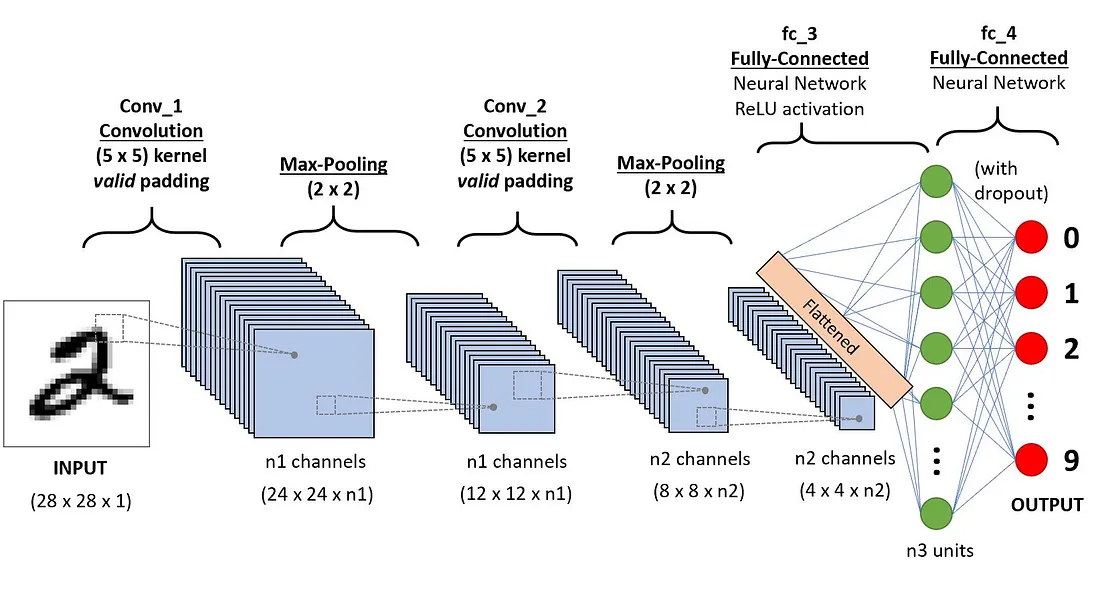
\includegraphics[width=0.5\textwidth]{Image/CNN.png}
    \caption{CNN}
    \label{fig:CNN}
\end{figure}

Nhờ khả năng học đặc trưng mạnh mẽ và hiệu quả tính toán cao, CNN được ứng dụng rộng rãi trong các bài toán nhận dạng ảnh, phân loại ảnh, phát hiện đối tượng, và các hệ thống thị giác máy tính.

\subsubsection*{4.2 RNN}
\addcontentsline{toc}{subsubsection}{RNN}

RNN là một kiến trúc mạng nơ-ron được thiết kế để xử lý dữ liệu tuần tự như văn bản, âm thanh, hoặc chuỗi thời gian. Khác với CNN, RNN có khả năng ghi nhớ thông tin từ các bước thời gian trước thông qua cơ chế lan truyền trạng thái ẩn (hidden state).

Tại mỗi bước thời gian, RNN nhận đầu vào mới cùng với trạng thái ẩn từ bước trước để cập nhật trạng thái hiện tại, cho phép mô hình xử lý các chuỗi dữ liệu có độ dài linh hoạt. Tuy nhiên, RNN truyền thống gặp khó khăn với hiện tượng tiêu biến hoặc bùng nổ gradient, dẫn đến việc ghi nhớ kém các thông tin dài hạn.

\begin{figure}[H]
    \centering
    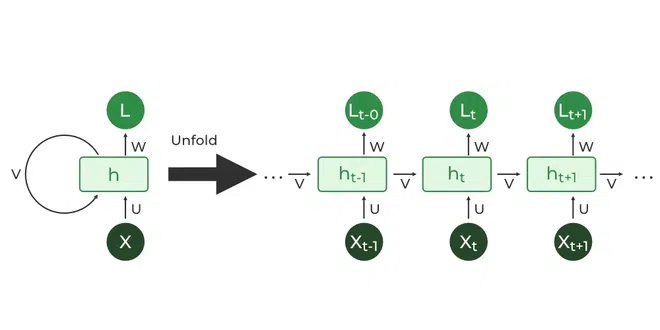
\includegraphics[width=0.5\textwidth]{Image/RNN.png}
    \caption{RNN}
    \label{fig:RNN}
\end{figure}

Do đó, trong thực tế, RNN thường được thay thế hoặc cải tiến bởi các kiến trúc mạnh hơn như LSTM hoặc GRU.

\subsubsection*{4.3 LSTM}

LSTM là một biến thể của RNN được thiết kế để giải quyết vấn đề quên thông tin dài hạn bằng cách sử dụng cơ chế “bộ nhớ” (memory cell). Mỗi đơn vị LSTM bao gồm ba cổng điều khiển: cổng vào (input gate), cổng quên (forget gate), và cổng đầu ra (output gate), cho phép mạng quyết định nên ghi nhớ, quên, hay xuất ra thông tin nào tại mỗi bước thời gian.

\begin{figure}[H]
    \centering
    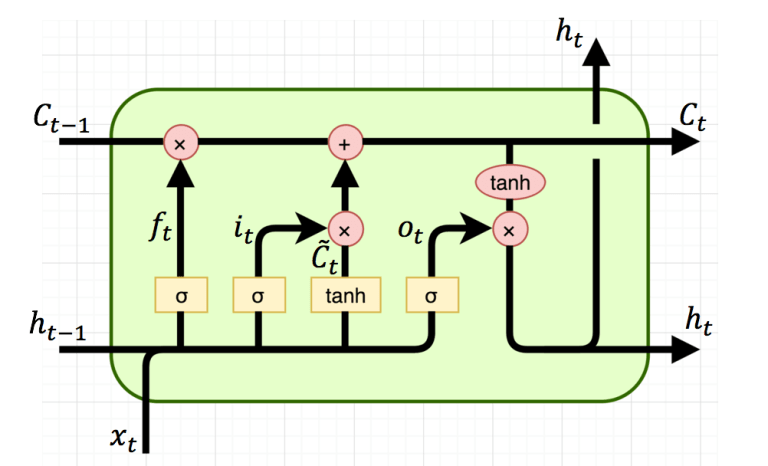
\includegraphics[width=0.5\textwidth]{Image/lstm.png}
    \caption{RNN}
    \label{fig:RNN}
\end{figure}

Điểm khác biệt giữa LSTM và RNN là LSTM có thể lưu trữ thông tin dài hạn hơn so với RNN thông qua các cổng ghi và đọc. Điều này giúp LSTM có thể xử lý chuỗi dữ liệu có độ dài lớn hơn so với RNN. Cơ chế này giúp LSTM duy trì được thông tin quan trọng trong thời gian dài, đồng thời tránh hiện tượng tiêu biến gradient khi huấn luyện. Nhờ đó, LSTM đặc biệt phù hợp với các bài toán liên quan đến ngôn ngữ tự nhiên, phân tích chuỗi thời gian, và dịch máy.

\subsubsection*{4.4 Transfer Learning}
\addcontentsline{toc}{subsubsection}{Transfer Learning}

Transfer Learning (học chuyển giao) là một kỹ thuật trong học máy, trong đó mô hình đã được huấn luyện trên một nhiệm vụ sẽ được tận dụng lại để áp dụng cho một nhiệm vụ mới có liên quan. Thay vì huấn luyện mô hình từ đầu với dữ liệu lớn, Transfer Learning cho phép tái sử dụng kiến thức đã học từ một mô hình gốc, đặc biệt hữu ích trong các bài toán có dữ liệu hạn chế.

Ý tưởng của học chuyển giao là khai thác các đặc trưng phổ quát đã được học trong một mô hình huấn luyện trước đó – chẳng hạn như các đặc trưng cạnh, hình dạng trong ảnh – và sau đó tinh chỉnh (fine-tune) mô hình này trên tập dữ liệu mục tiêu để đạt hiệu quả tốt mà không cần nhiều dữ liệu huấn luyện.

\begin{figure}[H]
    \centering
    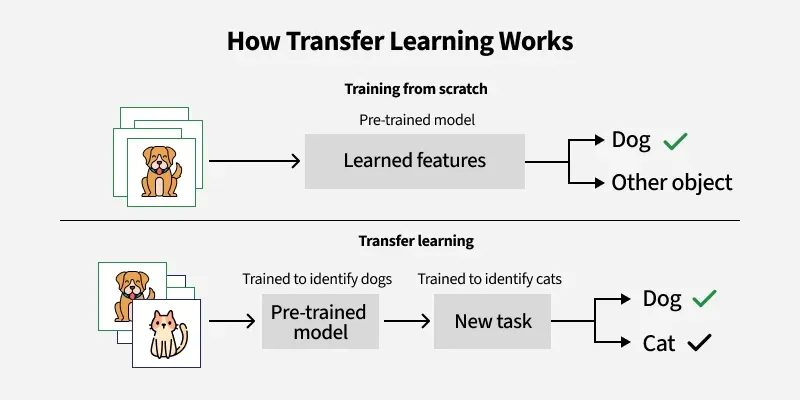
\includegraphics[width=0.75\textwidth]{Image/transfer-learning.png}
    \caption{Transfer Learning}
    \label{fig:Transfer Learning}
\end{figure}

Transfer Learning thường được thực hiện theo hai cách chính:

\begin{itemize}
    \item Feature Extraction: sử dụng mô hình đã huấn luyện để trích xuất đặc trưng, sau đó đưa vào một mô hình phân loại đơn giản như SVM hoặc một lớp fully connected.
    \item Fine-tuning: điều chỉnh một phần hoặc toàn bộ tham số của mô hình đã huấn luyện để phù hợp với dữ liệu mới.
\end{itemize}

Transfer Learning đã chứng minh hiệu quả vượt trội trong nhiều lĩnh vực như thị giác máy tính, xử lý ngôn ngữ tự nhiên và y sinh, đặc biệt khi dữ liệu mục tiêu khó thu thập hoặc có quy mô nhỏ. Nhờ khả năng tiết kiệm chi phí huấn luyện và cải thiện độ chính xác, Transfer Learning đã trở thành một chiến lược quan trọng trong thực tiễn ứng dụng học sâu hiện nay.


\subsubsection*{4.5 Mô hình CLIP}
\addcontentsline{toc}{subsubsection}{Mô hình CLIP}

CLIP (Contrastive Language-Image Pre-training) là một mô hình học sâu do OpenAI phát triển, được thiết kế để học cách biểu diễn hình ảnh và văn bản bằng cách so sánh chúng với các cặp ảnh–đoạn văn bản. Mô hình này được huấn luyện trên một tập dữ liệu lớn và được sử dụng để học cách biểu diễn hình ảnh và văn bản trong không gian vector.

\begin{figure}[H]
    \centering
    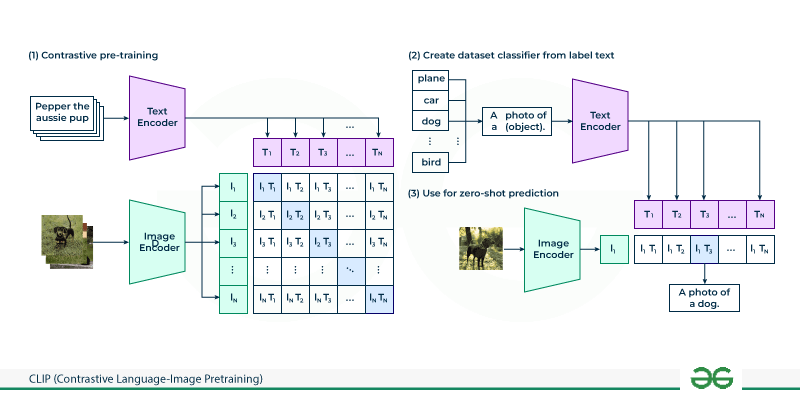
\includegraphics[width=1\textwidth]{Image/CLIP.png}
    \caption{CLIP}
    \label{fig:CLIP}
\end{figure}

CLIP sử dụng hai mạng neural riêng biệt: một mạng mã hóa hình ảnh (ví dụ ResNet hoặc Vision Transformer), và một mạng mã hóa văn bản (Transformer). Mỗi đầu vào được ánh xạ vào cùng một không gian nhúng, và mô hình học cách đưa các cặp tương ứng lại gần nhau, trong khi đẩy xa các cặp không tương ứng. Nhờ vào đó, CLIP có thể áp dụng cho nhiều tác vụ mà không cần huấn luyện lại, như tìm kiếm ảnh theo mô tả văn bản hoặc phân loại ảnh theo nhãn chưa từng thấy.

\subsubsection*{4.6 Cơ chế Attention}
\addcontentsline{toc}{subsubsection}{Cơ chế Attention}

Cơ chế Attention là một kỹ thuật trong học sâu cho phép mô hình tập trung vào những phần thông tin quan trọng trong đầu vào, thay vì xử lý toàn bộ thông tin một cách đồng đều. Cơ chế này được áp dụng rộng rãi trong các mô hình xử lý ngôn ngữ tự nhiên và thị giác máy tính.

\begin{figure}[H]
    \centering
    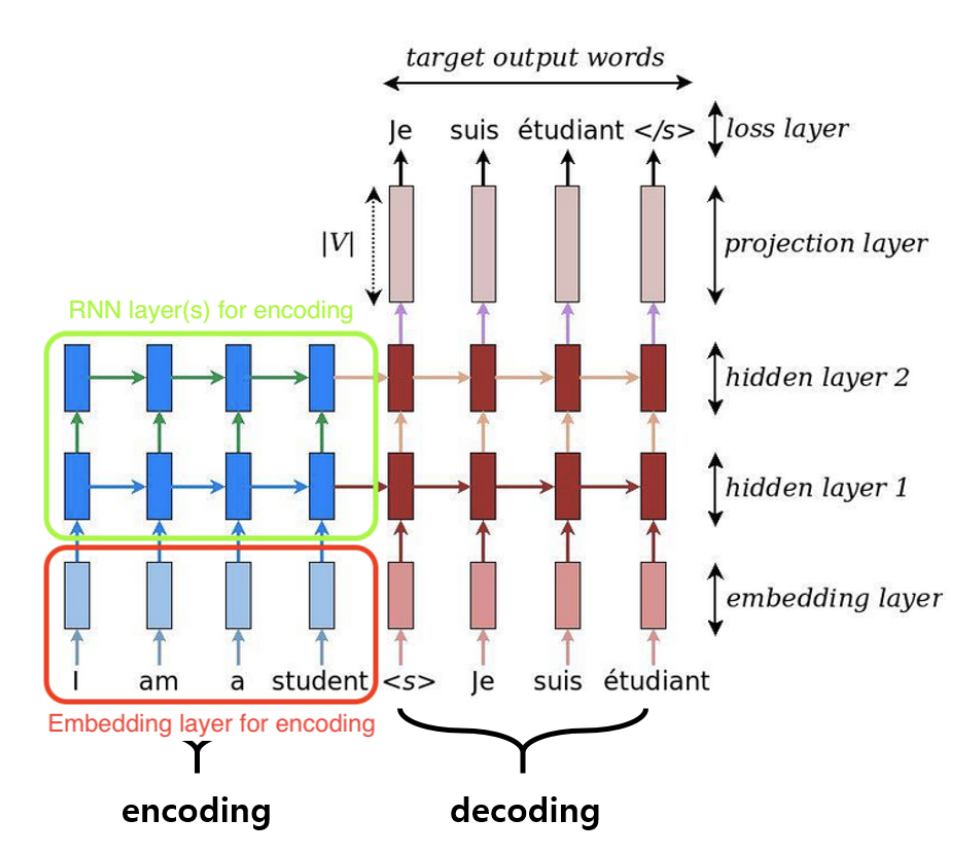
\includegraphics[width=1\textwidth]{Image/attention.png}
    \caption{Cơ chế Attention}
    \label{fig:Attention}
\end{figure}

Attention hoạt động bằng cách gán trọng số khác nhau cho từng phần tử đầu vào khi tính toán đầu ra. Điều này cho phép mô hình học được mối quan hệ giữa các từ trong câu hoặc các vùng trong ảnh, bất kể khoảng cách vị trí. Attention là thành phần cốt lõi trong kiến trúc Transformer, mở ra bước tiến lớn trong các ứng dụng như dịch máy, sinh văn bản và tổng hợp ngôn ngữ.

\subsubsection*{4.7 Beam Search}
\addcontentsline{toc}{subsubsection}{Beam Search}


Thuật toán này giúp cải thiện chất lượng sinh văn bản bằng cách tránh rơi vào lựa chọn tối ưu cục bộ. Beam Search thường được áp dụng trong các bài toán như dịch máy, sinh mô tả ảnh, và tổng hợp văn bản tự động.

\begin{figure}[H]
    \centering
    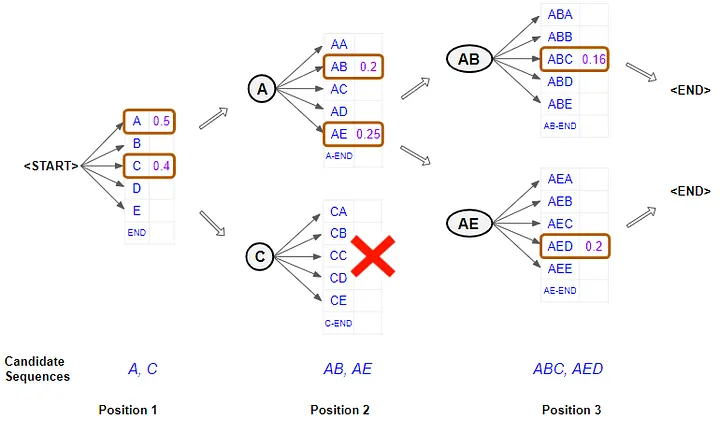
\includegraphics[width=1\textwidth]{Image/beamsearch.png}
    \caption{Beam Search}
    \label{fig:Beam Search}
\end{figure}

Công thức đánh giá xác suất chuỗi trong Beam Search:

$$
\log P(y | x) = \sum_{t=1}^{T} \log P(y_t | y_1, ..., y_{t-1}, x)
$$

Trong đó, mô hình sẽ chọn chuỗi đầu ra có tổng log xác suất cao nhất trong số các chuỗi được duy trì tại mỗi bước thời gian.

\subsubsection*{4.8 Chỉ số BLEU}
\addcontentsline{toc}{subsubsection}{Chỉ số BLEU}


BLEU (Bilingual Evaluation Understudy) là một phương pháp đánh giá tự động thường được sử dụng để đo lường chất lượng của các câu do mô hình dịch máy tạo ra bằng cách so sánh chúng với một hoặc nhiều câu tham chiếu được viết bởi con người. BLEU hoạt động dựa trên việc so khớp các n-gram giữa câu sinh ra và câu tham chiếu, từ đó tính toán điểm số thể hiện mức độ tương đồng.

Chỉ số BLEU được tính bằng trung bình hình học của độ chính xác n-gram (thường từ 1-gram đến 4-gram), kết hợp với một hệ số phạt (brevity penalty) nhằm điều chỉnh cho các câu sinh quá ngắn. Giá trị BLEU nằm trong khoảng từ 0 đến 1, trong đó giá trị càng cao thì chất lượng câu sinh ra càng gần với câu tham chiếu. Đây là thước đo phổ biến và hiệu quả trong việc đánh giá các mô hình sinh ngôn ngữ tự động.

Công thức tổng quát của BLEU như sau:

$$
\text{BLEU} = \text{BP} \cdot \exp\left( \sum_{n=1}^{N} w_n \log p_n \right)
$$

Trong đó:

\begin{itemize}
    \item $p_n$ là độ chính xác n-gram (precision) với n từ 1 đến N (thường là 4)
    \item $w_n$ là trọng số (thường đặt bằng nhau, $w_n = \frac{1}{N}$)
    \item $\text{BP}$ (brevity penalty) là hệ số phạt độ dài, được tính như sau
\end{itemize}

  $$
  \text{BP} = \begin{cases}
  1 & \text{nếu } c > r \\
  e^{(1 - \frac{r}{c})} & \text{nếu } c \leq r
  \end{cases}
  $$

  với $c$ là độ dài câu sinh, $r$ là độ dài tham chiếu gần nhất.


\end{document}